% Charles Haithcock 
% CSC 505, Steffen Heber
% Homework 2
% Due 24 February 2017

\documentclass{article}


%%%%%%%%%%%%%%%%%%%%%%%%%%%%%%%%%%%%%%%%%%%%%%%%%%%%%%%%%%%%%%%%%%%%%%%%%%%%%%%%
%                                   Packages                                   %
%%%%%%%%%%%%%%%%%%%%%%%%%%%%%%%%%%%%%%%%%%%%%%%%%%%%%%%%%%%%%%%%%%%%%%%%%%%%%%%%

\usepackage[utf8]{inputenc}
\usepackage{amsmath}            % Allows fancy math stuff
\usepackage{amssymb}            % Fancy math letters
\usepackage{graphicx}           % Allows for images
\usepackage[makeroom]{cancel}
\usepackage{framed}             % Allows boxes around text
\usepackage{parskip}            % Prevents paragraphs from being indented
\usepackage{minted}             % Allows pretty code blocks
\usepackage[margin=1.5in]{geometry} % Default margins make for tiny working 
                                % room for math. Make them smaller!


%%%%%%%%%%%%%%%%%%%%%%%%%%%%%%%%%%%%%%%%%%%%%%%%%%%%%%%%%%%%%%%%%%%%%%%%%%%%%%%%
%                                    Macros                                    %
%%%%%%%%%%%%%%%%%%%%%%%%%%%%%%%%%%%%%%%%%%%%%%%%%%%%%%%%%%%%%%%%%%%%%%%%%%%%%%%%

% Front Page macros
\newcommand{\homeworktitle}{\uppercase{Homework 3}}
\newcommand{\homeworkauthor}{Charles Haithcock}
\newcommand{\unityid}{cehaith2}
\newcommand{\duedate}{Due: 24 March 2017}
\newcommand{\coursetitle}{CSC 505 - Design and Analysis of Algorithms}
\newcommand{\instructor}{Steffen Heber}

% Other macros
\newcommand\floor[1]{\lfloor#1\rfloor}  % floor function decorators
\newcommand\ceil[1]{\lceil#1\rceil}     % ceiling function decorators
\newcommand\separator{\rule{\textwidth}{.2pt}}

%%%%%%%%%%%%%%%%%%%%%%%%%%%%%%%%%%%%%%%%%%%%%%%%%%%%%%%%%%%%%%%%%%%%%%%%%%%%%%%%
%                                   Title Page                                 %
%%%%%%%%%%%%%%%%%%%%%%%%%%%%%%%%%%%%%%%%%%%%%%%%%%%%%%%%%%%%%%%%%%%%%%%%%%%%%%%%

\begin{document}

\begin{center}
    \huge\textbf{\homeworktitle}
\end{center}
\vspace{1cm}

\begin{center}
    \large\homeworkauthor, \texttt{\unityid}
\end{center}
\vspace{1cm}

\begin{center}
    \large\coursetitle 
    
    \instructor
\end{center}
\vspace{1cm}

\begin{center}
    \large\duedate
\end{center}
\vspace{1cm}

\newpage



%%%%%%%%%%%%%%%%%%%%%%%%%%%%%%%%%%%%%%%%%%%%%%%%%%%%%%%%%%%%%%%%%%%%%%%%%%%%%%%%
%                                   Disclaimer                                 %
%%%%%%%%%%%%%%%%%%%%%%%%%%%%%%%%%%%%%%%%%%%%%%%%%%%%%%%%%%%%%%%%%%%%%%%%%%%%%%%%

Homework should be submitted using WolfWare Submit Admin in PDF, or plain text. 
To avoid reduced marks, please submit \textbf{word/latex-formated PDF file, NOT 
scanned writing in pdf format}. Scanned writing is hard to read, takes longer to
 grade, and produces gigantic files. \textbf{To simplify grading, please make 
sure that each problem starts on a new page}. All assignments are due on 9 PM of
the due date. Late submission will result in 10\%/40\% point reduction on the 
first/second day after the due date. No credit will be given to submission that 
are two or more days late. Please try out Submit Admin well before the due date 
to make sure that it works for you.

All assignments for this course are intended to be individual work. Turning in 
an assignment which is not your own work is cheating. The Internet is not an 
allowed resource! Copying of text, code or other content from the Internet (or 
other sources) is plagiarism. Any tool/resource must be approved in advance by 
the instructor and identified and acknowledged clearly in any work turned in, 
anything else is plagiarism.

General instruction about how to “give/describe/...” an algorithm, taken from 
Erik Demaine. \textbf{Try to be concise, correct, and complete.} To avoid 
deductions, you should provide (1) a textual description of the algorithm, and, 
if helpful, pseudocode; (2) at least one worked example or diagram to illustrate
how your algorithm works; (3) a proof (or other indication) of the correctness 
of the algorithm; and (4) an analysis of the time complexity (and, if relevant, 
the space complexity) of the algorithm. Remember that, above all else, your goal
is to communicate. If a grader cannot understand your solution, they cannot give
you appropriate credit for it.

\newpage

%%%%%%%%%%%%%%%%%%%%%%%%%%%%%%%%%%%%%%%%%%%%%%%%%%%%%%%%%%%%%%%%%%%%%%%%%%%%%%%%
%                                   Question 1                                 %
%%%%%%%%%%%%%%%%%%%%%%%%%%%%%%%%%%%%%%%%%%%%%%%%%%%%%%%%%%%%%%%%%%%%%%%%%%%%%%%%

\begin{framed}
    \textbf{Question 1 (4 pts)}
    
    Consider the coin-change problem from homework 2. Given a set of arbitrary 
    denominations $C =(c_1,...,c_d)$, describe an algorithm that uses dynamic 
    programming to compute the minimum number of coins required for making 
    change. You may assume that $C$ contains 1 cent.

    \separator

    \textit{Purpose} e) reinforce your understanding of dynamic programming and 
    the coin-change problem.

\end{framed}

%%%%%%%%%%
% Answer %
%%%%%%%%%%

\textbf{Answer}

See http://www.ccs.neu.edu/home/jaa/CSG713.04F/Information/Handouts/dyn_prog.pdf



\newpage




%%%%%%%%%%%%%%%%%%%%%%%%%%%%%%%%%%%%%%%%%%%%%%%%%%%%%%%%%%%%%%%%%%%%%%%%%%%%%%%%
%                                   Question 2                                 %
%%%%%%%%%%%%%%%%%%%%%%%%%%%%%%%%%%%%%%%%%%%%%%%%%%%%%%%%%%%%%%%%%%%%%%%%%%%%%%%%

\begin{framed}
    \textbf{Question 2 (14 pts total)}
    
    \begin{enumerate}
	\item[\textbf{a.}] \textbf{(12 pts.)} Implement a recursive, a dynamic 
	programming, and a memoized version of the algorithm for solving the 
	matrix-chain multiplication problem described in our textbook (Chapter 
	15), and design suitable inputs for comparing the run times, the number 
	of recursive calls, and the number of scalar multiplications for all 
	three algorithms. Describe the input data (tell us what inputs you used 
	and why these inputs are suitable for the desired measurments), tabulate 
	and plot your measurements and describe and comment your results. 
	Please submit your programs in three separate files: 
	\texttt{h3p2\_recursive\_uid.ext}, \texttt{h3p2\_dp\_uid.ext}, and 
	\texttt{h3p2\_memoized\_uid.ext}, where uid is your unity id and ext is
	the extension appropriate for your chosen programming language, e.g., 
	cpp for C++, java for Java, py for python, etc. Your report with graphs 
	and comments and a short description of how to run your program (on a 
	VCL Linux machine) should be submitted in a file called 
	\texttt{h3p2\_uid.pdf}.
        \item[\textbf{b.}] \textbf{(2 pts.)} Find an optimal parenthesization 
	of a matrix-chain product whose sequence of dimension is $<5, 2, 4, 7, 
	3, 9, 7, 8, 6, 3, 7, 5, 5>$. How many multiplications does this 
	parenthesization require? How many multiplications are required for a 
	parenthesization that multiplies the input matrices in their input 
	order?
    \end{enumerate}


    \separator

    \textit{Purpose} Reinforce your understanding of dynamic programming and 
    the matrix-chain multiplication problem, and practice run time measurements. 

\end{framed}


%%%%%%%%%%
% Answer %
%%%%%%%%%%

\newpage




%%%%%%%%%%%%%%%%%%%%%%%%%%%%%%%%%%%%%%%%%%%%%%%%%%%%%%%%%%%%%%%%%%%%%%%%%%%%%%%%
%                                   Question 3                                 %
%%%%%%%%%%%%%%%%%%%%%%%%%%%%%%%%%%%%%%%%%%%%%%%%%%%%%%%%%%%%%%%%%%%%%%%%%%%%%%%%

\begin{framed}
    \textbf{Question 3 (6 pts)}

    Let $G = (U, V, E)$ be a bipartite graph, i.e., a graph where the set of 
    vertices is partitioned into disjoint sets $U$ and $V$, and every edge 
    $(u,v)$ in $E$ has $u$ in $U$ and $v$ in $V$. Let $|V| < |U|$ and let 
    vertices in $U$ be numbered $1, \ldots , |U|$ and vertices in $V$ be 
    numbered $1, \dots , |V|$. The objective is to create a drawing of $G$ in 
    which
    \begin{enumerate}
        \item[(i)] the vertices of $U$ are mapped to integer coordinates $1, 
            \ldots , |U|$ on a horizontal line, no two vertices mapped to the 
            same coordinate; 
        \item[(ii)] the vertices of V are also mapped to coordinates $1, \ldots
            , |U|$ on a line above the one where the vertices of U appear, and 
            also, no two are mapped to the same coordinate;
        \item[(iii)] the vertices of both U and V appear left to right in 
            increasing numerical order; and 
        \item[(iv)] the edges are as “vertical as possible”. 
    \end{enumerate}
    
    To measure of how far away from vertical an edge between $i$ in $U$ and $j$
    in $V$ is we define \texttt{edgecost(i,j)} to be $(p(j) – i)^{2}$, where 
    $p(j)$ is the position of vertex $j$ on its horizontal line; note that the 
    positions of the vertices in $U$ are fixed. The picture below shows two 
    different drawings of the same graph $G$ and the computation of total cost 
    (i.e., the sum of all the edge costs) for each; costs for the edges 
    incident on each vertex of $V$ are grouped within parentheses, and the costs
    of individual edges appear in left to right order. The goal is to minimize 
    total cost.

    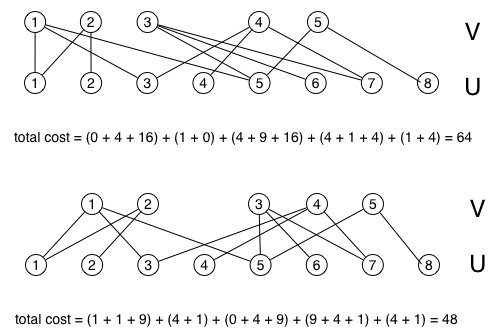
\includegraphics[width=\textwidth]{graph}

    If vertex $j$ of $V$ is placed in position $k$, we define 
    \texttt{vcost(j,k)} as the sum of edge costs of the edges incident on vertex
    $j$. In the above example, \texttt{vcost(1,1)} $= 0+4+16 = 20$, 
    \texttt{vcost(1,2)} $= 1+1+9 = 11$, \texttt{vcost(2,2)} $ =  1 + 0 = 1$, 
    \texttt{vcost(2,3)} $= 4 + 1 = 5$, \texttt{vcost(2,4)} $= 9 + 4 = 13$, and 
    \texttt{vcost(2,5)} $= 16 + 9 = 25$.

    Devise a dynamic programming algorithm to solve this problem. The runtime of
    your algorithm should be $\Theta(mn)$ where $m = |U|$ and $n = |V|$. You can
    assume that \texttt{vcost(j,k)} has  been precomputed for all relevant $j$ 
    and $k$ and can be retrieved in constant time. Your algorithm should report 
    both the cost of the minimum total cost drawing and the position of each 
    vertex in V in that drawing. Hint: Let $C[j,k]$ be the minimum total cost of
    a drawing for vertices $1, \ldots , j$ in $V$ that uses positions $1, \ldots
    , k$ only. Note that $C[j,k]$ is undefined for $j > k$ and for $k > |U| – 
    (|V| – j)$, and therefore \texttt{vcost(j,k)} is not used.

    \separator

    \textit{Purpose} Practice algorithm design and dynamic programming

\end{framed}

%%%%%%%%%%
% Answer %
%%%%%%%%%%

\textbf{Answer}



\newpage



\begin{framed}
    \textbf{Question 4 (6 pts)}
    
    Suppose you have a long straight country road with houses scattered at 
    various points far away from each other. The residents all want cell phone 
    service to reach their homes and we want to accomplish this by building as 
    few cell phone towers as possible.

    More formally, think of points $x_1, \ldots, x_n$, representing the houses, 
    on the real line, and let $d$ be the maximum distance from a cell phone 
    tower that will still allow reasonable reception. The goal is to find points
    $y_1,\ldots,y_k$ so that, for each $i$, there is at least one $j$ with 
    $|y_j - x_i | \le d$ and $k$ is as small as possible.

    Describe a greedy algorithm for this problem. If the points are assumed to 
    be sorted in increasing order your algorithm should run in time $O(n)$. Be 
    sure to describe the greedy choice and how it reduces your problem to a 
    smaller instance. Prove that your algorithm is correct.

    \separator

    \textit{Purpose} 
    Practice designing greedy algorithms.
\end{framed}

%%%%%%%%%%
% Answer %
%%%%%%%%%%

\textbf{Answer}

\textit{Textual description of the algorithm with pseudocode}

The algorithm takes as input \texttt{road}, a bitmask or list where 
\texttt{road[0]} is the first location on the road where a house could (or
could not) be and \texttt{road[n - 1]} is the last possible location. Where 
\texttt{road[i]} $= 1$, a house exists, and 0 otherwise.

To begin, the algorithm walks \texttt{road} to find the first house and records
the index. \texttt{road} is traversed further until the current location is 
distance $d$ away from the recorded index of the first house not covered by a 
tower or the end of the road is encountered. At this point, a tower is placed 
(the current index into \texttt{road} is recorded). The algorithm restarts at 
the point where it continues to walk to find the first house not covered by a 
tower. On termination, the list of tower indeces is returned.

\begin{minted}[
    framesep=2mm,
    baselinestretch=1.2,
    fontsize=\footnotesize,
    linenos
]{python}
def plot_towers(road, d):
    towers = [] 
    first = -1  # Index of first non-covered house

    for i in range(0, len(road)):

        # Mark index of first non-covered house
        if road[i] and first < 0:
            first = i
        
        # If placing a tower and d steps away from first house or at road end, 
        # record index and go back to searching for non-covered house
        if not first < 0 and (abs(i - first) == d or i == len(road) - 1:
            towers.append(i)
            first = -1

    return towers
\end{minted}

\textit{A worked example}

Assume \texttt{road} $= \{0, 0, 1, 0, 1, 0, 0, 1\}$ and $d = 3$. The 
algorithm walks starting from index 0 until index 2 is encountered as the first
non-covered house. \texttt{first} then becomes 2 and the algorithm continues
until index 5. At this point, $|i - d| = $ \texttt{first} so \texttt{towers} $=
\{5\}$. From here, \texttt{roads} is traversed further for the next non-covered 
house. However, the list end is reached before another house is found, so 
$\{5\}$ is returned. 

In the above example, the coverage of houses can not be done with fewer towers
as fewer towers is 0. As such, the solution is also the optimal solution which 
minimizes the amount of towers necessary while covering all houses. 

\textit{Proof}

Maybe proof by contradiction? The professor went over this in class. Go to the
greedu algorithm lectures to get the proof. 

\textit{Time complexity analysis}

All lines in the pseudocode are constant time operations, $\Theta(1)$. However, 
line 5 is a loop walking the length of \texttt{road} and is therefore executed
$n$ times. As such, line 5 through 15 execute $n$ times. Each of the loop body 
statements are constant time, so the complexity is dominated by the loop
executing $n$ times. Furthermore, because the loop will always run $n$ times, 
complexity is then $\Theta(n)$. 

Some considerations for this algorithm include future expansions to the road and
representation of the \texttt{road} input. For example, if houses will be built,
the placements may no longer be optimal. Likewise, if the \texttt{road} is a bit
mask, \texttt{road} can be segmented and each segment be checked to have values
above 0. While the asymptotic complexity will not improve from $\Theta(n)$, the
amortized analysis could potentially be closer to $\Theta(\log(n))$ for more 
sparse roads. Heavily populated roads, however, would likely end up devolving 
into something along the lines of $\Theta(mn)$ where $m$ is the amount of
segments. 



\newpage






\end{document}
